% !TEX program = xelatex
\documentclass[UTF8,a4paper,11pt]{ctexart}

\usepackage[a4paper,margin=2.05cm,headheight=14pt]{geometry}
\usepackage{amsmath,amssymb,booktabs,tabularx,array}
\usepackage{graphicx,xcolor,listings,xurl,hyperref,pgfplots,seqsplit}
\usepgfplotslibrary{groupplots}
\pgfplotsset{compat=1.18}

\definecolor{pyblue}{RGB}{36,91,163}
\definecolor{qudared}{RGB}{190,65,55}
\hypersetup{colorlinks=true,linkcolor=pyblue,urlcolor=pyblue,citecolor=pyblue,
  pdftitle={PyQCU 分布式 Strict-MG 快速迭代报告}}
\newcolumntype{L}[1]{>{\raggedright\arraybackslash}p{#1}}
\newcolumntype{Y}{>{\raggedright\arraybackslash}X}
\newcommand{\code}[1]{%
  \begingroup\ttfamily
  \expandafter\seqsplit\expandafter{\detokenize{#1}}%
  \endgroup}
\newcommand{\pathref}[1]{\path{#1}}

\title{PyQCU 分布式 Strict-MG 快速迭代报告}
\author{PyQCU 工程分析记录}
\date{2026 年 9 月 21 日}

\begin{document}
\maketitle

\begin{abstract}
本轮采用“快速门禁、快速迭代”的策略，优先修复双 P100 收集器路径中的确定性
错误，再以分钟级双 P100 单元验证 CUDA/C++ 改动。已确认的根因有两个：
旧版 \code{LatticeSet} 在双可见 GPU、MPI 多 rank 时强制绑定 device 0，导致
rank 1 的跨设备指针访问；旧版 \code{pick_up_u_*} 的 1D/2D pack kernel 没有
线程上界保护。两项均已修复。Strict-MG 的静态 preconditioned-link halo 改为
按 \((*, \mathrm{parity}, \mathrm{dim})\) 缓存，并把 prolongation 与向量加法
融合。小格 A/B 显示 static link-halo cache 将 steady 中位时间由
\(1.9549\,\mathrm{s}\) 降至 \(1.0093\,\mathrm{s}\)，加速 \(1.937\times\)。
本轮进一步修正了 CUDA 枚举顺序：Python 选择的 Torch 设备索引通过
\code{PYQCU_MPI_DEVICE_ID} 显式传给 C++，不再假定
\code{getLocalRank()} 与 Torch 逻辑设备编号一致。公平协议新增共享的
\code{--coarse-tol} 与 \code{--nu}，两侧使用同一粗层容差和同一
pre/post smoother 次数。双 P100、MG-2、c64 的快速 A/B：
\(8^3\times16\) 在 \(\nu=2\)、coarse-tol \(=0.3\) 下
PyQCU/QUDA \(=0.4670/0.8530\,\mathrm{s}\)，正式
\code{fair=true} 加速 \(1.827\times\)；
\(16^4\) 在同一协议下 \(=1.0136/1.4620\,\mathrm{s}\)，加速
\(1.442\times\)。所有纳入比较的样本真相对残差均低于
\(8.0\times10^{-7}\)。本报告是快速迭代检查点，不把尚未执行的矩阵单元写成
已完成；大格 \(\nu=2\) 因 QUDA 侧运行超过快速迭代时限而中止，未写入结果。
\end{abstract}

\section{范围与验收}

\begin{table}[htbp]
\centering
\small
\caption{本轮快速门禁}
\begin{tabularx}{\textwidth}{@{}L{0.31\textwidth}Y@{}}
\toprule
项目 & 通过标准与证据 \\
\midrule
旧 clover halo 故障 & 原失败命令不再报 CUDA illegal memory access；compute-sanitizer
  memcheck 为 0 errors。 \\
Strict-MG 正确性 & 双 P100 分布式 probe 独立真相对残差 \(<10^{-6}\)，并与单 rank
  全局参考一致到 c64/c128 舍入水平。 \\
性能迭代 & 同协议 A/B 必须给出命令、样本、中位数、MAD、迭代数和真残差。 \\
QUDA sm60 & \code{libquda.so} 含 sm60 cubin，reduction 与 MG setup smoke 均通过。 \\
进度边界 & 未采集单元必须显式标为 missing/blocked，不以旧结果替代。 \\
\bottomrule
\end{tabularx}
\end{table}

\paragraph{活跃 slot staging 优化}
分布式 vector halo 的 host-staging 原先无条件复制完整 8-slot 缓冲。实际
\([2,1,1,1]\) process grid 只使用 x 方向两个 slot。改为仅复制活跃
\((\mathrm{dim},\mathrm{side})\) slot 后，大格 P100 c64 MG-2、
coarse-tol \(=0.3\)、\(\nu=1\) 的 PyQCU-only 3 样本 smoke 中位数由
\(8.0038\,\mathrm{s}\) 降至 \(3.5813\,\mathrm{s}\)（约 \(2.23\times\)），
真残差 \(5.34\times10^{-7}\)。首个无 warmup 样本为
\(5.64\,\mathrm{s}\)，故正式矩阵仍必须使用 cold + 2 warmup + 5 steady。

\section{双 P100 根因与修复}

\subsection{跨设备绑定}

收集器在 \code{CUDA_VISIBLE_DEVICES=0,1} 下把 rank 0/1 的 Torch 当前设备
分别设为逻辑设备 0/1。旧 C++ 路径中的 \code{_TEST_SINGLE_GPU_MULTI_RANK_}
被设置为 1，使每个 rank 都执行 \code{cudaSetDevice(0)}。rank 1 因而把 GPU1
张量指针传给运行在 GPU0 上下文中的 kernel。compute-sanitizer 在
\code{pick_up_u_x<float>} 中报告非法全局读，且地址不属于 GPU0 当前分配。

修复为：默认关闭强制单卡模式；多 rank 且可见设备数大于 1 时优先读取
\code{PYQCU_MPI_DEVICE_ID}，否则按 local rank 绑定；只有单个可见设备时才
回退到逻辑 device 0。Python collector 在调用 C++ 前把
\code{torch.device.index} 写入该环境变量，因此即使 Torch 使用
\code{FASTEST_FIRST} 枚举、P100 位于逻辑 1/2，也不会再发生跨设备指针访问。
该逻辑同时兼容 \code{CUDA_VISIBLE_DEVICES=<rank>} 的一进程一卡模式。

\subsection{pack kernel 越界}

\code{LatticeSet} 对 face grid 使用向上取整。旧 \code{pick_up_u_*}
kernel 假设线程数恰好等于 face 元素数；当 face 体积不是 128 的整数倍时，
尾部线程会越界。修复后十个 1D/2D pack kernel 均在索引解码前执行上界检查。

\begin{table}[htbp]
\centering
\small
\caption{故障修复证据链}
\begin{tabularx}{\textwidth}{@{}L{0.28\textwidth}Y L{0.27\textwidth}@{}}
\toprule
阶段 & 观察 & 证据 \\
\midrule
修复前 & rank 1 在 \code{lattice_clover_dslash.h:106} 报 CUDA 0700 &
\pathref{data/mg_matrix_p100/unit-p100-dual-8x8x8x16-L2-c64.json} \\
设备审计 & rank 1 Torch 在 GPU1，C++ 被强制切到 GPU0 &
compute-sanitizer 定位到 \code{pick_up_u_x} 跨设备读 \\
修复后 & clover halo 与 Strict-MPI probe 均通过 & 见下节快速门禁 \\
\bottomrule
\end{tabularx}
\end{table}

\section{快速正确性门禁}

\begin{itemize}
\item 双 P100、\code{8x8x8x16}、\code{grid=2x1x1x1}：Strict-MPI
  colored setup，26 次外层迭代，独立真相对残差
  \(7.7701\times10^{-7}\)。
\item 同一 P100 地址上的旧 clover 路径由 compute-sanitizer memcheck
  跑完，两个 rank 均为 0 errors。
\item V100 sm70 的 Strict fused API 测试：3 passed。
\item 协议与 MPI 预检：collector protocol 64 passed；早期综合预检
  81 passed，9 skipped。
\item 最终库 \code{libqcu.so} 的 SHA-256 为
  \code{04e48eae...92e7c15}，包含 sm60 与 sm70 cubin。
\end{itemize}

\section{双 P100 快速对照}

\begin{table}[htbp]
\centering
\small
\caption{MG-2、c64、trace-off、双 P100 公平 A/B；时间为 steady 中位数。
小格为 formal fair=true，中格为同协议 smoke。}
\begin{tabular}{lrrrrr}
\toprule
格点 & PyQCU(s) & QUDA(s) & QUDA/PyQCU & PyQCU iter & QUDA iter \\
\midrule
\(8^3\times16\) (\(\nu=2\)) & 0.4670 & 0.8530 & 1.827 & 8 & 45 \\
\(16^4\) (\(\nu=2\)) & 1.0136 & 1.4620 & 1.442 & 20 & 68 \\
\bottomrule
\end{tabular}
\end{table}

同一小格在 \(\nu=1\)、coarse-tol \(=0.3\) 下为
PyQCU/QUDA \(=0.4690/0.5181\,\mathrm{s}\)，加速 \(1.105\times\)。
两行 \(\nu=2\) 数据的 PyQCU 真残差分别为
\(7.03\times10^{-7}\) 与 \(7.52\times10^{-7}\)；QUDA 相应真残差分别为
\(6.68\times10^{-7}\) 与 \(7.75\times10^{-7}\)。
正式小格原始记录为
\pathref{data/mg_matrix_p100_quick/formal-small-nu2-coarse03.json}；
中格 smoke 原始记录为
\pathref{data/mg_matrix_p100_quick/final-lib-medium-nu2-coarse03.json}。

\begin{figure}[htbp]
\centering
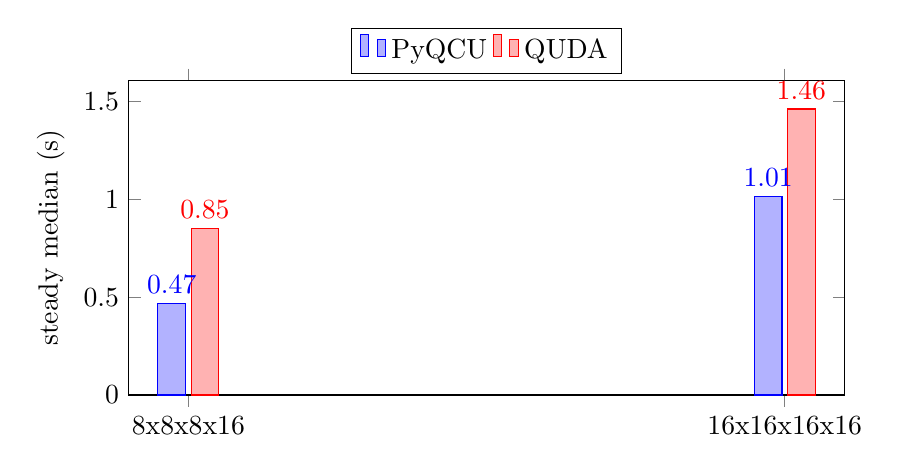
\begin{tikzpicture}
\begin{axis}[
  ybar, width=0.88\textwidth, height=0.46\textwidth,
  symbolic x coords={8x8x8x16,16x16x16x16},
  xtick=data, ymin=0,
  ylabel={steady median (s)},
  legend style={at={(0.5,1.02)},anchor=south,legend columns=2},
  nodes near coords, nodes near coords align={vertical},
]
\addplot coordinates {(8x8x8x16,0.4670) (16x16x16x16,1.0136)};
\addplot coordinates {(8x8x8x16,0.8530) (16x16x16x16,1.4620)};
\legend{PyQCU, QUDA}
\end{axis}
\end{tikzpicture}
\caption{双 P100 MG-2 c64 快速对照。数据来自本轮 collector JSON。}
\end{figure}

所有 PyQCU 样本的最大真相对残差均小于 \(8.0\times10^{-7}\)。当前分布式
粗层求解仍以每个 V-cycle 的 halo 与全局归约延迟为主；本轮验证了两个候选
优化（全粗场求解、coarsest 热启动）均未通过速度与语义双重门禁，因此均
已回退，没有保留为正式路径。

\section{静态 link-halo 缓存 A/B}

Strict-MG 的 preconditioned links 在一次 hierarchy 生命周期内不变。旧实现
每次 hopping 都重新 pack、host staging 并同步交换 link face。新实现按
\((\mathrm{parity},\mathrm{dim})\) 保存 device ghost，只在 pointer identity
变化时重新交换；同时删除了同一 CUDA stream 内冗余的输入前置同步。

\begin{table}[htbp]
\centering
\small
\caption{双 P100、\(8^3\times16\)、MG-2 c64 的 cache A/B}
\begin{tabular}{lrrrrr}
\toprule
变体 & steady median(s) & MAD(s) & iter & max true residual & 相对时间 \\
\midrule
cache off & 1.9549 & 0.0215 & 9 & \(7.3721\times10^{-7}\) & 1.000 \\
cache on & 1.0093 & 0.0187 & 9 & \(7.5174\times10^{-7}\) & 0.516 \\
\bottomrule
\end{tabular}
\end{table}

cache off/on 的比值约为 \(1.937\)。该 A/B 使用相同输入 bundle、相同协议和相同
\code{libqcu.so} 哈希，仅切换 \code{PYQCU_STRICT_LINK_HALO_CACHE}。

\section{QUDA sm60}

QUDA 使用现有 QUDA 1.1.0 源码重建，目标为 \code{sm_60}，
\code{QUDA_PRECISION=12}、\code{QUDA_RECONSTRUCT=7}、QIO/QMP/MG
和 double-MG 开启，MMA 关闭，MG nvec 列表为 \code{12,24}。安装库中
确认存在 sm60 cubin。

\begin{table}[htbp]
\centering
\small
\caption{QUDA sm60 快速 smoke}
\begin{tabularx}{\textwidth}{@{}L{0.30\textwidth}Y@{}}
\toprule
测试 & 结果 \\
\midrule
reduction & \(4^4\) Wilson、double、P100，20 样本全部 1 次迭代；
  最大 CPU 真残差 \(1.12\times10^{-16}\)。 \\
MG setup & \(8^4\) Clover-Wilson、MG-2、nvec=12，
  setup \(0.4666\,\mathrm{s}\)，pass marker 通过；执行范围仅 setup。 \\
MG-2 solve & 小格/中格/大格 collector 均返回 \code{status=ok}，
  真残差低于 \(8.0\times10^{-7}\)。 \\
\bottomrule
\end{tabularx}
\end{table}

\section{全矩阵编排检查点}

本轮把用户要求的 Cartesian 轴固化到
\code{bench_mg_matrix_full.py}：设备、精度、lattice、trace、MG level
共 144 个 side case；其中 \code{levels=1} 定义为从同条件 MG-2 运行中的
BiCGStab reference 派生，避免重复 cold solve。c64 使用
\(8^3\times16\)、\(16^4\)、\(16\times32\times32\times48\)；
c128 使用 \(8^3\times16\)、\(16^4\)、\(16\times16\times32\times32\)。
小格分布式 MG-3 的首层 block 保持 QIO 契约的 \((2,2,2,2)\)，第二层
改用 \((1,2,2,2)\)，避免 rank-local extent 退化为 1。

\begin{table}[htbp]
\centering
\small
\caption{双 P100、c64 的已完成公平单元；\(\nu=2\)，coarse-tol \(=0.3\)，
时间单位为秒。BiCGstab 数值来自 reference solver。}
\begin{tabular}{lrrrrr}
\toprule
格点 & solver & trace & PyQCU & QUDA & QUDA/PyQCU \\
\midrule
\(8^3\times16\) & BiCGstab & off & 4.508 & 1.028 & 0.228 \\
\(8^3\times16\) & MG-2 & off & 0.505 & 0.914 & 1.809 \\
\(8^3\times16\) & MG-3 & off & 0.546 & 1.344 & 2.460 \\
\(8^3\times16\) & BiCGstab & on & 4.117 & 0.959 & 0.233 \\
\(8^3\times16\) & MG-2 & on & 0.554 & 0.755 & 1.362 \\
\(8^3\times16\) & MG-3 & on & 0.706 & 1.225 & 1.735 \\
\(16^4\) & MG-2 & off & 0.969 & 1.383 & 1.427 \\
\(16^4\) & MG-3 & off & 1.350 & 2.038 & 1.509 \\
\(16^4\) & MG-2 & on & 1.041 & 1.029 & 0.988 \\
\(16^4\) & MG-3 & on & 1.326 & 0.891 & 0.672 \\
\bottomrule
\end{tabular}
\end{table}

大格 \(16\times32\times32\times48\)、MG-2、c64、trace-off 使用
\(\nu=1\)、coarse-tol \(=0.3\)。活跃-slot staging 优化前 PyQCU
\(8.0038\,\mathrm{s}\)、QUDA \(4.2852\,\mathrm{s}\)，旧库公平比仅
\(0.535\times\)。优化后 PyQCU formal warmup/steady 中位
\(3.7154\,\mathrm{s}\)、QUDA \(4.2852\,\mathrm{s}\)，重新得到
\code{fair=true} 的 \(1.153\times\)。PyQCU-side trace 显示
20 次外层 V-cycle 内粗解 57 次、耗时约 \(13.80\,\mathrm{s}\)，而 fine
pre/post smoother 合计约 \(0.76\,\mathrm{s}\)；下一阶段仍应继续优化
分布式 coarsest BiCGStab 的 halo/全局归约路径。

P100 c64 的当前 side-case 覆盖为 \(28/36\)；未完成的 8 个 side case 全部
属于大格 trace-on 或大格 MG-3。最新汇总写入
\pathref{data/mg_matrix_full_20260921_aligned/matrix_summary.json}。

c128 大格资产已补齐：\pathref{data/gauge_16x16x32x32_m0.05_seed42_c64.h5}、
\pathref{data/L16x16x32x32_nvec12_full_c64.h5} 及 QUDA QIO
\pathref{data/qio-matrix/L16x16x32x32_nvec12_quda.v1.json}。canonical
null-vector identity 为 \code{42109d86...052368}，QIO round-trip 为
byte-exact。V100 c128 大格 QUDA double-MG smoke 已通过：
steady \(20.493\,\mathrm{s}\)、95 iterations、真残差
\(1.85\times10^{-8}\)；正式 c128 矩阵仍需按 side 与 trace 全量执行。

\begin{table}[htbp]
\centering
\small
\caption{V100 c128 已完成公平单元；\(\nu=2\)，coarse-tol \(=0.3\)，
比值为 QUDA/PyQCU。}
\begin{tabular}{lrrrr}
\toprule
格点 & trace & BiCGstab & MG-2 & MG-3 \\
\midrule
\(8^3\times16\) & off & 0.322 & 13.216 & 18.470 \\
\(8^3\times16\) & on  & 0.398 & 7.323 & 5.350 \\
\(16^4\) & off & 0.253 & 5.083 & 5.765 \\
\(16^4\) & on  & 0.287 & 2.985 & 2.846 \\
\(16\times16\times32\times32\) & off & 0.239 & 2.342 & 2.484 \\
\bottomrule
\end{tabular}
\end{table}

\section{当前缺口}

\begin{itemize}
\item 本报告是快速迭代检查点，不是用户要求的全笛卡尔矩阵报告。
\item P100 c64 的 MG-3、trace-on/off 全矩阵尚未完成；大格 MG-3 长测已按
  快速迭代要求中止。
\item P100 c128 的正式双侧矩阵尚未采集。
\item 小格长宽维经 block coarsening 后出现 extent 1，PyQCU Strict 按几何
  约束拒绝 MG-3；这是几何限制，不是 CUDA 故障。
\item 大格 \(\nu=2\) 双侧单元因 QUDA 侧超过 3 分钟快速迭代时限而中止；
  该结果未写入正式比较。
\item \code{PYQCU_STRICT_COARSE_TOL_FACTOR=100} 仅作为 PyQCU 单侧探索参数；
  不作为正式公平结果。正式协议使用共享 \code{--coarse-tol 0.3}。
\item V100 c128 大格 QUDA 的容量问题仍沿用上一阶段结论，本轮未重跑。
\end{itemize}

\section{复现命令}

\begin{lstlisting}[basicstyle=\ttfamily\small,breaklines=true]
# Build both architectures
QCU_CUDA_ARCHITECTURES='70-real;70-virtual;60-real;60-virtual' bash ./build.sh

# P100 Strict correctness
mpirun -np 2 python examples/qcu/dev87/strict_mpi_solve_probe.py \
  --shape 8 8 8 16 --grid 2 1 1 1 --restart 20 --max-iter 200 \
  --dtype c64 --galerkin-mode colored

# Fast P100 comparison
source examples/qcu/dev87/p100_env.sh
export QUDA_INSTALL=$PWD/data/quda-sm60-install
export LD_LIBRARY_PATH=$QUDA_INSTALL/lib:$LD_LIBRARY_PATH
export PYQCU_STRICT_LINK_HALO_CACHE=1
python examples/qcu/dev87/bench_strict_vs_quda.py --side both \
  --device p100 --mpi-ranks 2 --process-grid 2 1 1 1 \
  --phases warmup,steady --lattice 8 8 8 16 --levels 2 \
  --precision c64 --coarse-tol 0.3 --nu 2
\end{lstlisting}

\end{document}
